%%%%%%%%%%%%%%%%%%%%%%%%%%%%%%%%%%%%%%%%%%%%
% arara: pdflatex: { synctex: on }
% arara: pdflatex: { synctex: on }
\documentclass[oneside]{scrbook}

\usepackage[utf8]{inputenc}
\usepackage{polski}
%\usepackage{identfirst}
 \usepackage{amsfonts}
\usepackage{amsmath}
\usepackage{amsthm}
\usepackage{enumitem}
\usepackage[all,cmtip]{xy}

\usepackage{graphicx}
\usepackage{caption}
\usepackage{tikz}
\usetikzlibrary{shapes.geometric, arrows}
\usepackage{mathtools, stackengine}
\usepackage{amsfonts}


\title{Języki formalne i złożoność obliczeniowa.}
\author{Na podstawie wykładu profesora Macieja Kandulskiego}
\date{semestr zimowy 2019/2020}


\titlehead{Notatki z wykładu Pani Sarenki}
\publishers{Uniwersytet Adama Mickiewicza wydział Matematyki i Informatyki}

\begin{document}
\maketitle

%\frontmatter
%\tableofcontents
%\listoffigures
%\listoftables

%\chapter{Acknowledgements}

%I would like to thank my supervisor, Professor Someone. This
%research was funded by the Imaginary Research Council.

%\chapter{Abstract}

%A brief summary of the project goes here.

%\mainmatter

\backmatter
\chapter{Wykład 12.10.2019}
\label{ch:wyklad1}

\section{Złożoność obliczeniowa}

Zagadnienia złożoności obliczeniowej
- jakie sa koszty prowadzenia obliczeń czasowe i pamięciowe:
\begin{itemize}
  \item Złożoność wykładnicza
  \item Nierozsądne gospodarowanie czasem
  \item Nierozsądne gospodarowanie pamięciową \ldots
\end{itemize}


\section{Gramatyka}

\newtheorem*{theorem*}{Gramatyka}
\begin{theorem*} Jak poprawnie budować wyrażenia danego języka (zbiór zasad).
Gramatyka inaczej jest nazywana syntaktyką albo składnią. \end{theorem*}



%schemat gramatyki
\begin{tikzpicture}

\node[draw, rectangle, minimum width = 3 cm, minimum height = 2 cm] (fl) at (0,0) { \bf JĘZYK};


% oznaczenie nad dgłównym prostokatem 
%\node[above] at (fl.north) {$V(B)$};

\draw[<-] (fl) -- node[above]{ \bf gramatyka} node[below]{generowanie wyrażeń} ++(-6,0);
\draw[<-] (fl) -- node[above]{\bf automat} node[below]{rozpoznawanie wyrażeń tego języka} ++(8,0);
\end{tikzpicture}


Między innymi kompilator posiada w sobie element rozpoznający gramatykę. \newline


%%%%%%%%%%%%%%%%%%%%%% Symbol %%%%%%%%%%%%%%%%%%%%


\section{Symbol a znaczenie symbolu}

 \subsection{Abstrakcyjne pojęcie liczby}


Warto odróżnić symbol od jego znaczenia. Np. liczbę dwa można zapisywac w postaci symoblu cyfry arabskiej { \bf 2} lub rzymskiej  { \bf II}. To samo dotyczy słowa { \bf słoń } - słowo oznacza wielkie kilkutonowe zwierze ale nim nie jest (nie jest bytem materialnym). 

\newtheorem*{theorem2*}{Abstrahować}
\begin{theorem2*} Abstrachować znacyz pomijać. Np.: abstrakcyjna liczba dwa powstała z pominięciem takich cech jak wielkość, pochodzenie.
 \end{theorem2*}
 
\subsection{Przykład powstania liczby}
Różna materialne nośniki niosące te same liczby obiektów o różnych cechach.Opisanie wspólnej cechy obiektów - { \bf liczebności} .

 
\begin{enumerate}[label=(\roman*)]
  \item {\bf couple} of people (para ludzi - 2)
  \item {\bf pair} of pistols (para pistoletów - 2)
  \item {\bf yoke} of oxen (zaprzęg dwa zwięrzęta)
\end{enumerate}
 
 

Abstakcyjna liczba { \bf 2} powstała abstrahując od pochodzenia (np. zwierzęcia), wielkości (np. broni) czy płci (para ludzi) pozostawiając tylko jedną wspólną cechę, którą jest { \bf liczebność} . 
 

%%%%%%%%%%%%%%%%%%%%%% języki formalne %%%%%%%%%%%%%%%%%%%%

\section{Języki formalne}
\subsection{Pojęcia}

Ciągi i zbiory ciągów traktowane są jako obiekty materialne a { \bf nie } abstrakycjne. \newline
{ \bf Skończoność} - ważna cecha alfabetu/zbioru ponieważ tylko skończone zbiory danych można przechowywać w { \bf fizycznym urządzeniu}. 

\newtheorem*{theorem3*}{Alfabet V}
\begin{theorem3*} Alfabet V to: { \bf dowolny} , { \bf niepusty} , { \bf skończony zbior znaków}  \newline np.: V = \{I\} , V' = \{a,b\}.
\newline


 \end{theorem3*}


\newtheorem*{theorem4*}{Słowo nad alfabetem V}
\begin{theorem4*} Słowo nad alfabetem V to dowolny, skończony ciąg znkaów z V. np.: {\bf IIII} (słowo nad alfabete V=\{I\}) czy {\bf abba} (słowo nad alfabetem V=\{a,b\}) 
 \end{theorem4*}


\newtheorem*{theorem5*}{Słowo puste $\epsilon$}
\begin{theorem5*}Słowo puste $\epsilon$ - słowo o 0 (zerowym) wystąpieniu symboli. Uwaga! Spacja {\bf NIE} jest słowem pustym.
 \end{theorem5*}
 
 
 \newtheorem*{theorem6*}{V*}
\begin{theorem6*}Zbiór wszsytkich słów nad alfabetem V. Łącznie z pustym słowem $\epsilon$.
 \end{theorem6*}
 
 
\newtheorem*{theorem7*}{V* \textbackslash \{$\epsilon$\} = V+}
\begin{theorem7*}
Zbiór wszsytkich niepustych słów. (ŁWyłączenie ze zbioru pustego słowa $\epsilon$)
 \end{theorem7*}
 
\newtheorem*{theorem8*}{Oznaczenie słów}
\begin{theorem8*}
Słowa oznaczane są wielkimi literami z końca alfabetu łacińskiego, np.: { \bf P},{\bf Q},{\bf R}. 
 \end{theorem8*}
 

\subsection{Operacja konkatenacji}

\newtheorem*{theorema*}{Konkatenacja dwóch słów}
\begin{theorema*}
Konkatenacją dwóch słów {\bf P} i {\bf Q} nazywamy słowo {\bf PQ} zdefiniowane w następujący sposób:

\begin{enumerate}[label=(\roman*)]
  \item jeżeli {\bf P}=$a_{1}, ... ,a_{n}$ gdzie {\bf a}=$b_{1}, ... ,b_{n}$ n,m $\ge$ 0 to {\bf PQ}= $a_{1},...,a_{n}b_{1},...,b_{n}$
  \item Jeżeli {\bf P}=$\epsilon$, to {\bf PQ}=Q.\newline 
  Alternatywnie to {\bf Q}=$\epsilon$ i wtedy {\bf PQ}=P. \newline
  Gdy {\bf P}={\bf Q}=$\epsilon$ to {\bf PQ=}$\epsilon\epsilon$ = $\epsilon$ . 
\end{enumerate} 

 
 \end{theorema*}



\subsubsection{Własności konkatenacji}
\begin{itemize}
  \item Konkatenacja jest działaniem łacznym w zbiorze słów
  \item Konkatenacja w ogólnoście {\bf NIE} jest przemienna (bywa przemienna dla tyh samych słów {\bf ab} {\bf ab } ) lub jeśli alfabet skada sie tylko z jednego znaku np V = \{a\}
  \item $\epsilon$ słowo puste zachowje się jak element neutralny dla operacji konkatenacji: \newline $\epsilon$P $\subset$ 
  P$\epsilon$ = P.
\end{itemize}


\subsection{Konkatenacja NIE jest grupą algebraiczną  $\heartsuit$}
Pomimo abstrakcyjnego znaczenia liczb, ich mentalna reprezentacja jest jednak w urządzeniu czymś materialnym (stanami wysokich i niskich napięć).

 $V^{*}$ - zbiór wszystkich elementow (słów) nad alfabatem { \bf V} (łącznie z elementem pustym $\epsilon$)

$\circ$ - oznacza działanie w grupie 

{\bf e} - litera e jest symbolem elementu neutralnego \newline

Przykład łączności:
a) dodawanie np. : 2 + (3 + 5) = (2 + 3) + 5
b) mnożenie np.:  2 * (3 * 5) = (2 * 3) * 5
 
Konkatenacja jest grupą (z algebry) jeśli spełnia warunki na bycie grupą:


\begin{enumerate}[label=(\roman*)]
  \item operacja $\circ$ jest łączna w grupie;
  \item $\exists e$, $\forall x $ Istnieje element neutralny dal każdego x, taki że  $x \circ e = e \circ x = x$;
  \item Dla każdego x $\forall x $   Istnieje element odwrotny  $\exists x^{-1}$, taki, że  $x \circ  x^{-1} = x^{-1} \circ x = e$. \newline Warunek nie spełniony przez konkatenację - nie istnieje w ogólności takie słowo gdzie: słowo + słowo$^{-1} = \epsilon$ 
  (szczególny przypadek spełnienia to $\epsilon$ + $\epsilon$ = $\epsilon$, bo element neutralny jest sam do siebie odwrotny $\epsilon^{-1} = \epsilon$ ) \newline $\Rightarrow$ {\bf WARUNEK NIE JEST W OGÓLNOŚCI SPEŁNIONY - konkatenacja NIE jest grupą!}
\end{enumerate}


\subsection{Podsłowo słowa}
Zbiór { \bf A } $\subset$   { \bf A } i analogicznie  { \bf abca } $\sqsubset$  { \bf abca }
(Znak $\sqsubset$  to taka kanciasta inkluzja oznaczenie używane przy słowach)


\newtheorem*{theorem9*}{Podsłowo}
\begin{theorem9*}
Mówimy, że słowo {\bf Q} jest podsłowem słowa {\bf P} wtedy i tylko wtedy gdy, istnieją słowa $Q_{1}$ i $Q_{2}$ takie, że:
\begin{center}
$P = Q_{1}${\bf Q}$Q_{2}$.
\end{center}
Np:. słowo {\bf bc} jest podsłowem słowa {\bf abcd} 


\begin{center}
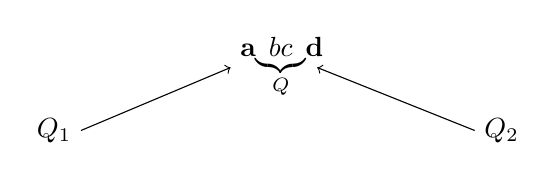
\begin{tikzpicture}
\node[left]{$Q_{1}$};
\draw[->] (0,0)-- (1.9,0.8) node[right]{{\bf a}$\underbrace{bc}_{Q}${\bf d}};
\draw[<-] (3,0.8) -- (5,0) node[right]{$Q_{2}$};
\end{tikzpicture}
\end{center}

Widać, tutaj, zę Q to słowo {\bf ab}, $Q_{1} = a$, $Q_{2}=d$
\end{theorem9*}
 

\newtheorem*{theorem10*}{Prefix słowa}
\begin{theorem10*}
Słowo $Q$ jest prefixem słowa $P$ jeśli $P = QQ_{1}$.
\end{theorem10*}
 
\newtheorem*{theorem11*}{Suffix słowa}
\begin{theorem11*}
Słowo $Q$ jest suffixem słowa $P$ jeśli $P =Q_{1}Q$.
\end{theorem11*}

\newtheorem*{theorem12*}{Infix słowa}
\begin{theorem12*}
Słowo $Q$ jest infixem słowa $P$ jeśli $P =Q_{1}QQ_{2}$  \newline
gdzie $Q_{1}\neq \epsilon$ i gdzie $Q_{2} \neq \epsilon$.
\end{theorem12*}



\subsection{Długość słowa}
\newtheorem*{theorem13*}{Długość słowa $\mid P\mid$}
\begin{theorem13*}
Długością słowa $P \subset V^{*}$ nazywamy liczbę naturalną $\mid P\mid$ definiujemy w sposób indukcyjny:
 
\begin{enumerate}[label=(\roman*)]
  \item $ \mid  \epsilon \mid=0$
  \item $ \mid P{ \bf a}  \mid= \mid P \mid + 1$; gdzie P to ciąg (słowo) a {\bf a} to symbol (dodatkowa litera w słowie).
\end{enumerate} 
 
\end{theorem13*}


\paragraph{Przykład 1.}
Długość słowa {\bf abc} \newline
$\mid abc \mid = \mid ab \mid + 1 = ( \mid a \mid + 1) + 1 = 
(\mid \epsilon a \mid + 1) + 1 =   ((\mid \epsilon \mid + 1 )+1)+1 =
((0+1)+1)+1 = 3
$ 

\paragraph{Przykład 2.}
Obliczyć ilość wszystkich podsłów słowa {\bf P} gdy dana jest długość słowa $\mid P \mid = 4$ \newline
Odp: { \bf NIE WIĘCEJ NIŻ} 11. \newline
Rozwiązanie a):\newline
Weźmy dla przykładu słowo {\bf abcd }. 

Podsłowo {\bf abcd} $\subset$ {\bf abcd} - jedno podsłowo długości 4. (Słowo jest samo swoim podsłowem; kolejnosć znaków też ma znaczenie np słowo {\bf bcda} $\not\subset $ {\bf abcd}  ).
\newline

Podsłowa długości 3 (2 takie słowa)
{\bf abc} $\subset$ {\bf abcd},
{\bf bcd} $\subset$ {\bf abcd};

Podsłowa długości 3 (2 takie słowa)
{\bf ab} $\subset$ {\bf abcd},
{\bf bc} $\subset$ {\bf abcd},
{\bf cd} $\subset$ {\bf abcd};

Podsłowa długości 1 (4 takie słowa)
{\bf a} $\subset$ {\bf abcd},
{\bf b} $\subset$ {\bf abcd},
{\bf c} $\subset$ {\bf abcd},
{\bf d} $\subset$ {\bf abcd};

Odp a) Dla słowa { \bf abcd} mamy (1+2+3+4) + 1( dodajemy jeden bo znak pusty $\epsilon$ )

Rozwiązanie b):
Załóżmy, że szukamy wszystkich podsłów słowa P = {\bf aaaa}. 
aaaa $\subset$  aaaa (1 podsłowo)
aaa $\subset$  aaaa (1 podsłowo)
aa $\subset$  aaaa (1 podsłowo)
a $\subset$  aaaa (1 podsłowo)

Odp a) Dla słowa { \bf aaaa} mamy (1+1+1+1) + 1( dodajemy jeden bo znak pusty $\epsilon$ ), ponieważ {\bf NIE ROZRÓŻNIAMY ZNAKÓW MIĘDZY SOBĄ tzn.: zawsze a == a} (nie rozróżniamy permutacji tych samych elementów)


\paragraph{Zadanie Domowe na ćwiczenia}
Napisać procedurę w pseudokodzie:
Dla zadanego słowa długośc {\bf n} napisac procedurę, które pokaże liczbę {\bf k} podsłów oraz wypisze całą listę konkretnych podsłów.

\subsection{Długość konktatenacji słów}

\newtheorem*{theorem14*}{Długość konktatenacji słów}
\begin{theorem14*}
\begin{center}
$\mid PQ \mid = \mid P \mid + \mid Q \mid$
\end{center}

Dowód (indukcja matematyczna):\newline
$\forall P,Q: \mid PQ \mid = \mid P \mid + \mid Q \mid$ (Indukcja po długości $\mid Q \mid$)

\begin{enumerate}[label=(\roman*)]
\item $\mid Q \mid = \epsilon$ \newline
LewaStrona: $\mid PQ \mid = \mid P \epsilon \mid = \mid P \mid$ \newline
PrawaStrona: $\mid P \mid + \mid Q \mid = \mid P \mid + \mid \epsilon \mid = \mid P \mid+ 0 = \mid P \mid $ = { \bf LewaStrona} 
\newline c.n.d (co należało dowieść)
  
  
\item $\mid PQ \mid = \mid P \mid + \mid Q \mid $ \newline
PrawaStrona: $\mid P(Qa) \mid = \mid P \epsilon \mid = \mid P \mid$ \newline

LewaStrona: $\mid P \mid + \mid Q \mid = \mid P \mid + \mid \epsilon \mid = \mid P \mid+ 0 = \mid P \mid $ = { \bf LewaStrona} \newline c.n.d (co należało dowieść)
  
\end{enumerate} 
\end{theorem14*}






%%%%%%%%%%%%%%%%%%%%%%%%%%%%%%%%%%%%%%%%%%%%%%%%%%%%%

\newpage
\chapter{Brudnopis}
\label{ch:brudnopis}

$$\heartsuit$$

$\underbrace{wyr1}_{wyr2},\overbrace{wyr1}^{wyr2}$

$\exists y\geq 0\;\forall x:x\leq y$

 $\sqsupset$ 
 
 
 \begin{tikzpicture}
\draw[->] (0,0) node[left]{Q} -- (2,1) node[right]{abcd} -- (3,1)(5,0) node[right]{Q2};


\end{tikzpicture}


\xymatrix{
    A \ar[d] \ar[dr] \ar[drr] &   &   \\
    B                         & C & D }

\xymatrix{A &*+[F]{\sum_{i=n}^m {i^2}} \\& {\bullet} & D \ar[ul]     }

\xymatrix{A \ar[d]^b \ar[r]^a &B\ar[d]^c\\C \ar[r]^d          &D}



\begin{picture}(300,20)
\put(50,10){\vector(2,-3){20}}
\put(50,10){\vector(2,-1){60}}
\put(-10,15){these guys \textbf{here} must be eliminated. The next one \textbf{here} too, of course.}
\put(230,10){\vector(-2,-3){20}}
\end{picture}
\[ \bigl\{ \underbracket[0.5pt]{x \in \mathbb{Z}}_{\clap{\footnotesize Menge aller $x$ aus $\mathbb{Z}$}} \stackrel{\Shortstack {\clap{\footnotesize mit der Eigenschaft}\\$\downarrow $}}{\mid} -1 \le x \le 2\bigr\} \]
\\[1cm]
And I want to get it like this:
\[ \{x \in \mathbb{Z} \ | \ -1 \le x \le 2 \}, \]
where the \verb|\overbrace| doesn't wait till the \verb|\underbrace| is going to have the work done.



%\backmatter

\end{document} 